% vim:ts=4:sw=4
% Copyright (c) 2014 Casper Ti. Vector
% Public domain.

\chapter{原型系统的设计与实现}
	\section{系统架构}
		高速公路关键路段识别算法是为了解决高速公路管理者解决高速公路资源配比问题而开发的,整个系统基于B/S架构,从高层划分为前端和后端两部分,具体系统架构见图\ref{fig20},后端为Windows服务,主要包括实时车辆数据的处理以及数据仓库的存储。前端系统中,我们编写自己的业务逻辑,Web Service和展现系统,通过调用已有的数据访问层进行数据处理,完成系统任务。

		\begin{figure}[h]
		\centering
				\begin{minipage}{0.8\linewidth}
					\centering
					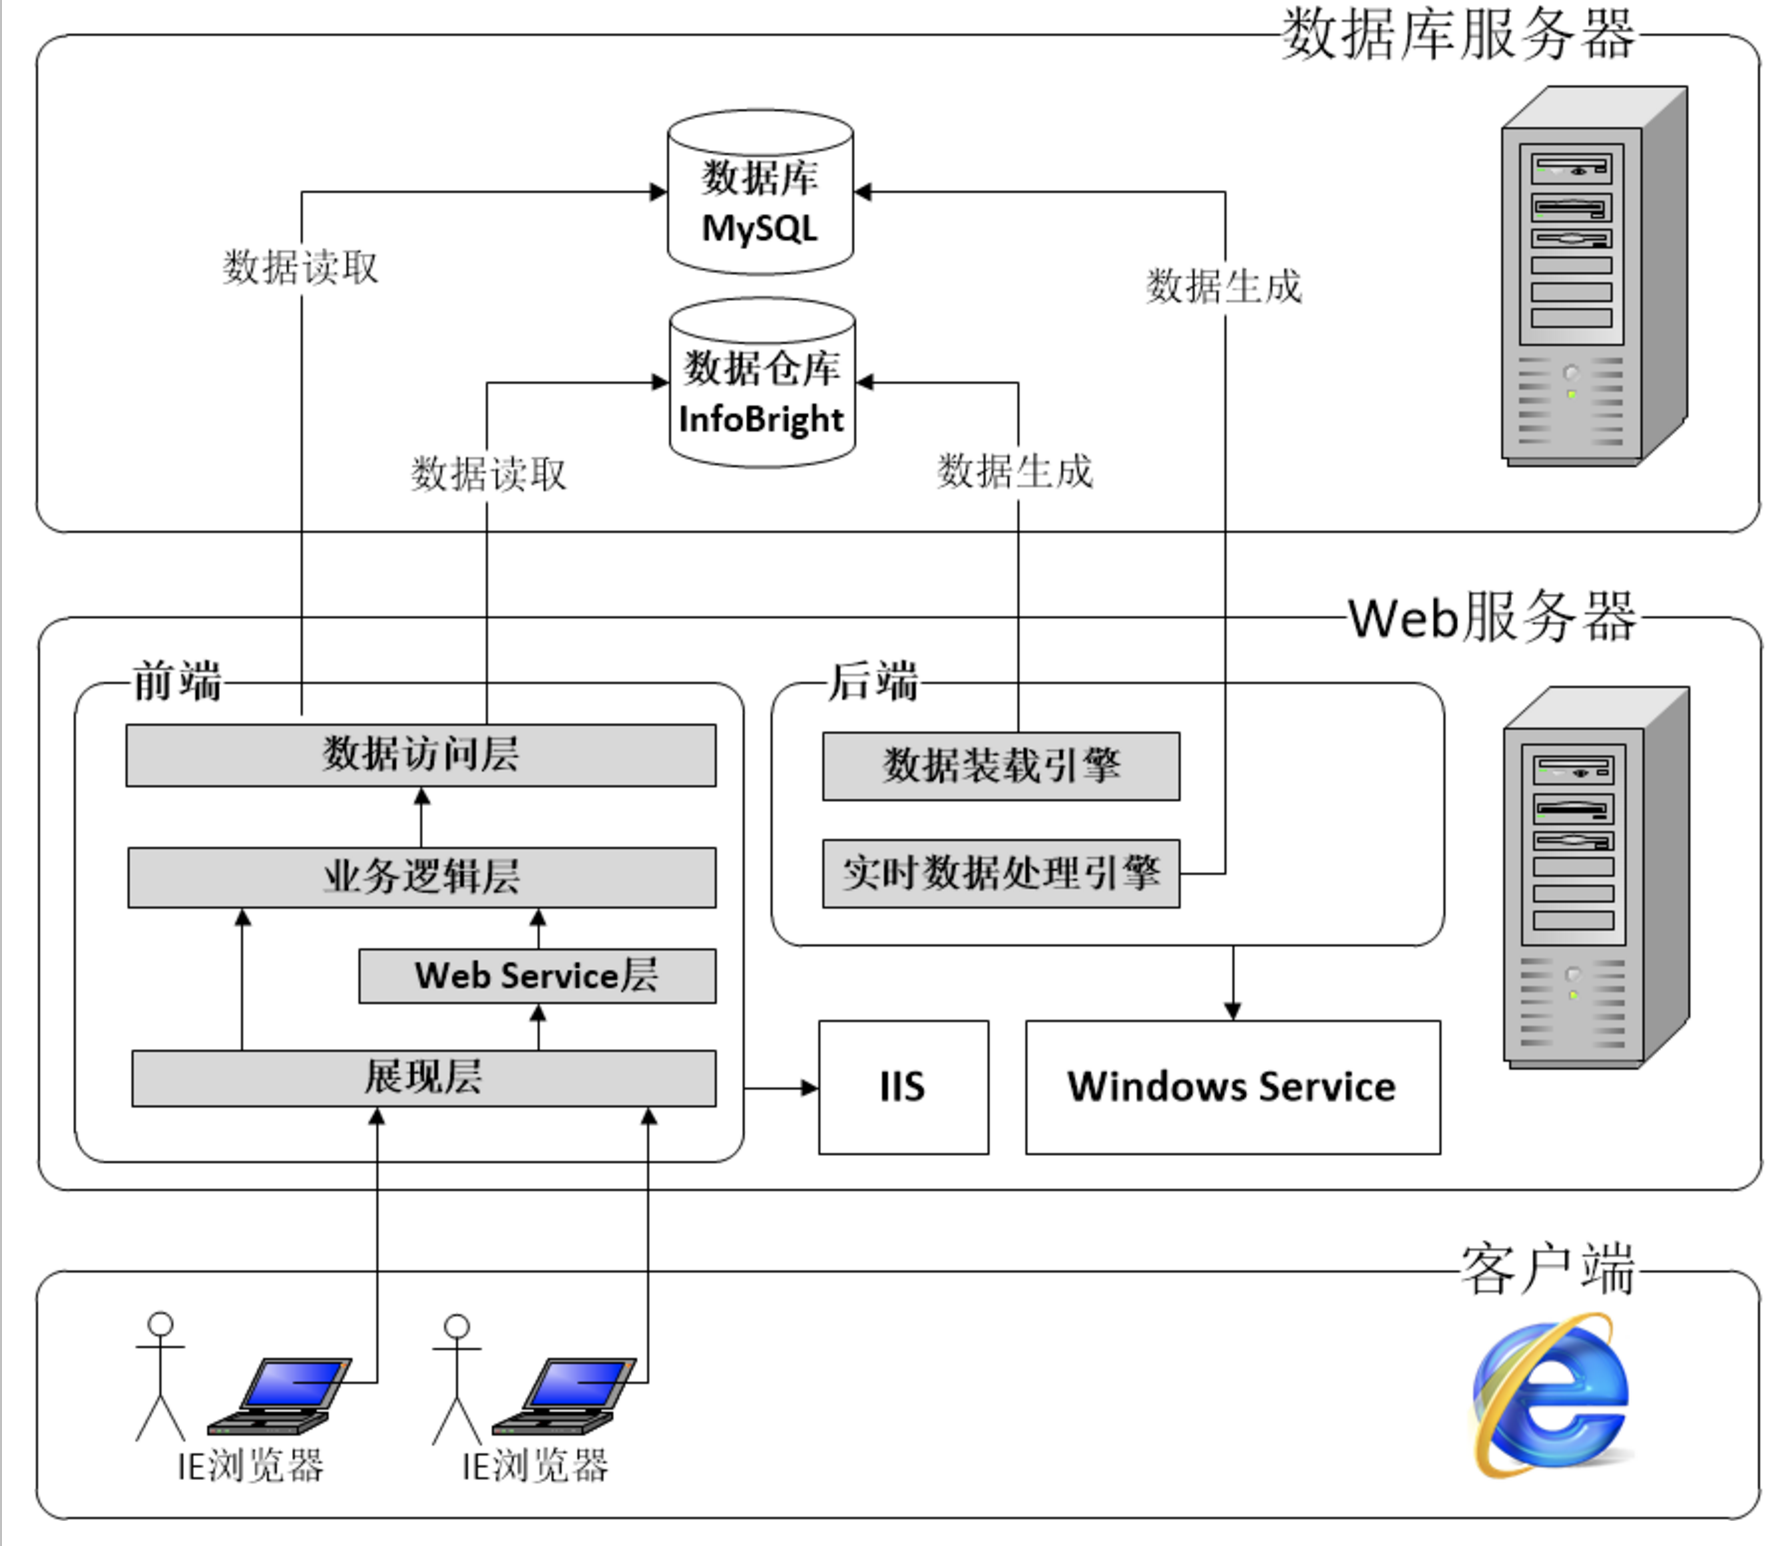
\includegraphics[width=4.4in]{picture/jiagou}
					\caption{fig1}
					\label{fig20}
				\end{minipage}%\
		\end{figure}
	\section{结合高速公路分群算法的并行策略}
		系统中,采用hadoop中的map reduce思想,进行效率优化。首先在主机器中进行分群,然后将每一个社群数据map到子机器中,在子机器中计算社群内部的关键节点,之后将结果reduce到主机器中,计算出最终结果。

		流程图见图\ref{mapreduce}:
		\begin{figure}[h]
		\centering
				\begin{minipage}{0.8\linewidth}
					\centering
					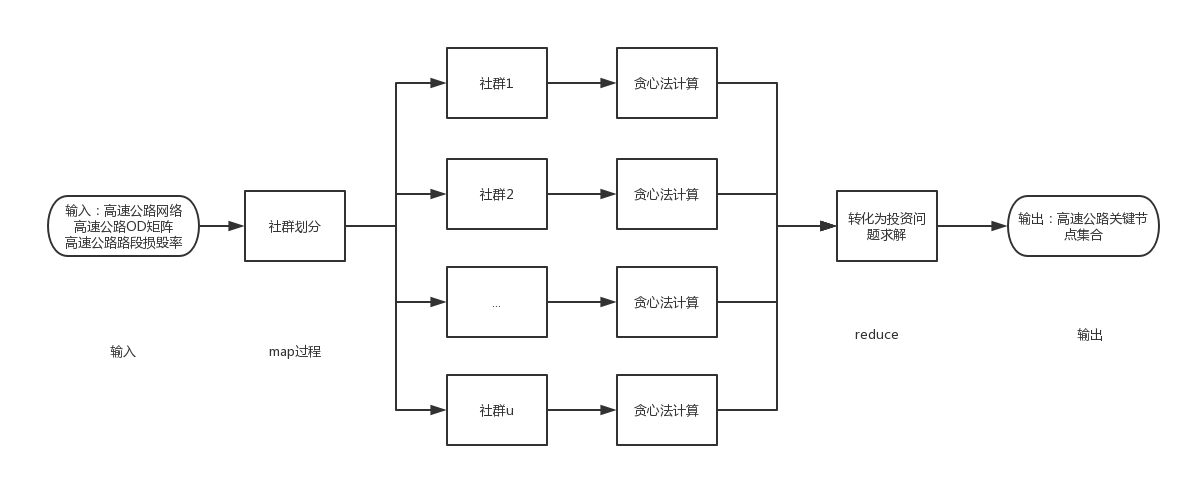
\includegraphics[width=4.4in]{picture/mapreduce}
					\caption{fig1}
					\label{mapreduce}
				\end{minipage}%\
		\end{figure}

	\section{系统模块}

		系统主要面向高速公路上重大事故的预防与处理。与城市路网相比,高速公路联网收费数据能够获得准确的用户OD数据,可以有效的进行分析。图\ref{fig21}是关键路段挖掘系统的技术流程图。

		\begin{figure}[h]
		\centering
				\begin{minipage}{0.8\linewidth}
					\centering
					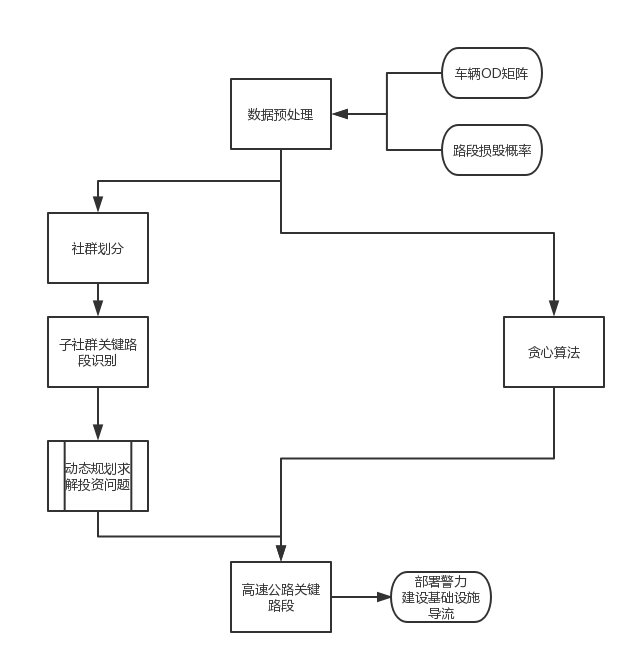
\includegraphics[width=4.4in]{picture/liuchengtu}
					\caption{fig1}
					\label{fig21}
				\end{minipage}%\
		\end{figure}
		
	\section{界面功能展示}

		系统的输入有时间,时间区间,路段损毁概率,管理者对关键路段的维护效果。

		系统输出两层信息,第一层是关键路段分群效果,如图\ref{yuanxing1};第二层是关键路段选取结果,如图\ref{yuanxing2}。

		\begin{figure}[h]
		\centering
				\begin{minipage}{0.8\linewidth}
					\centering
					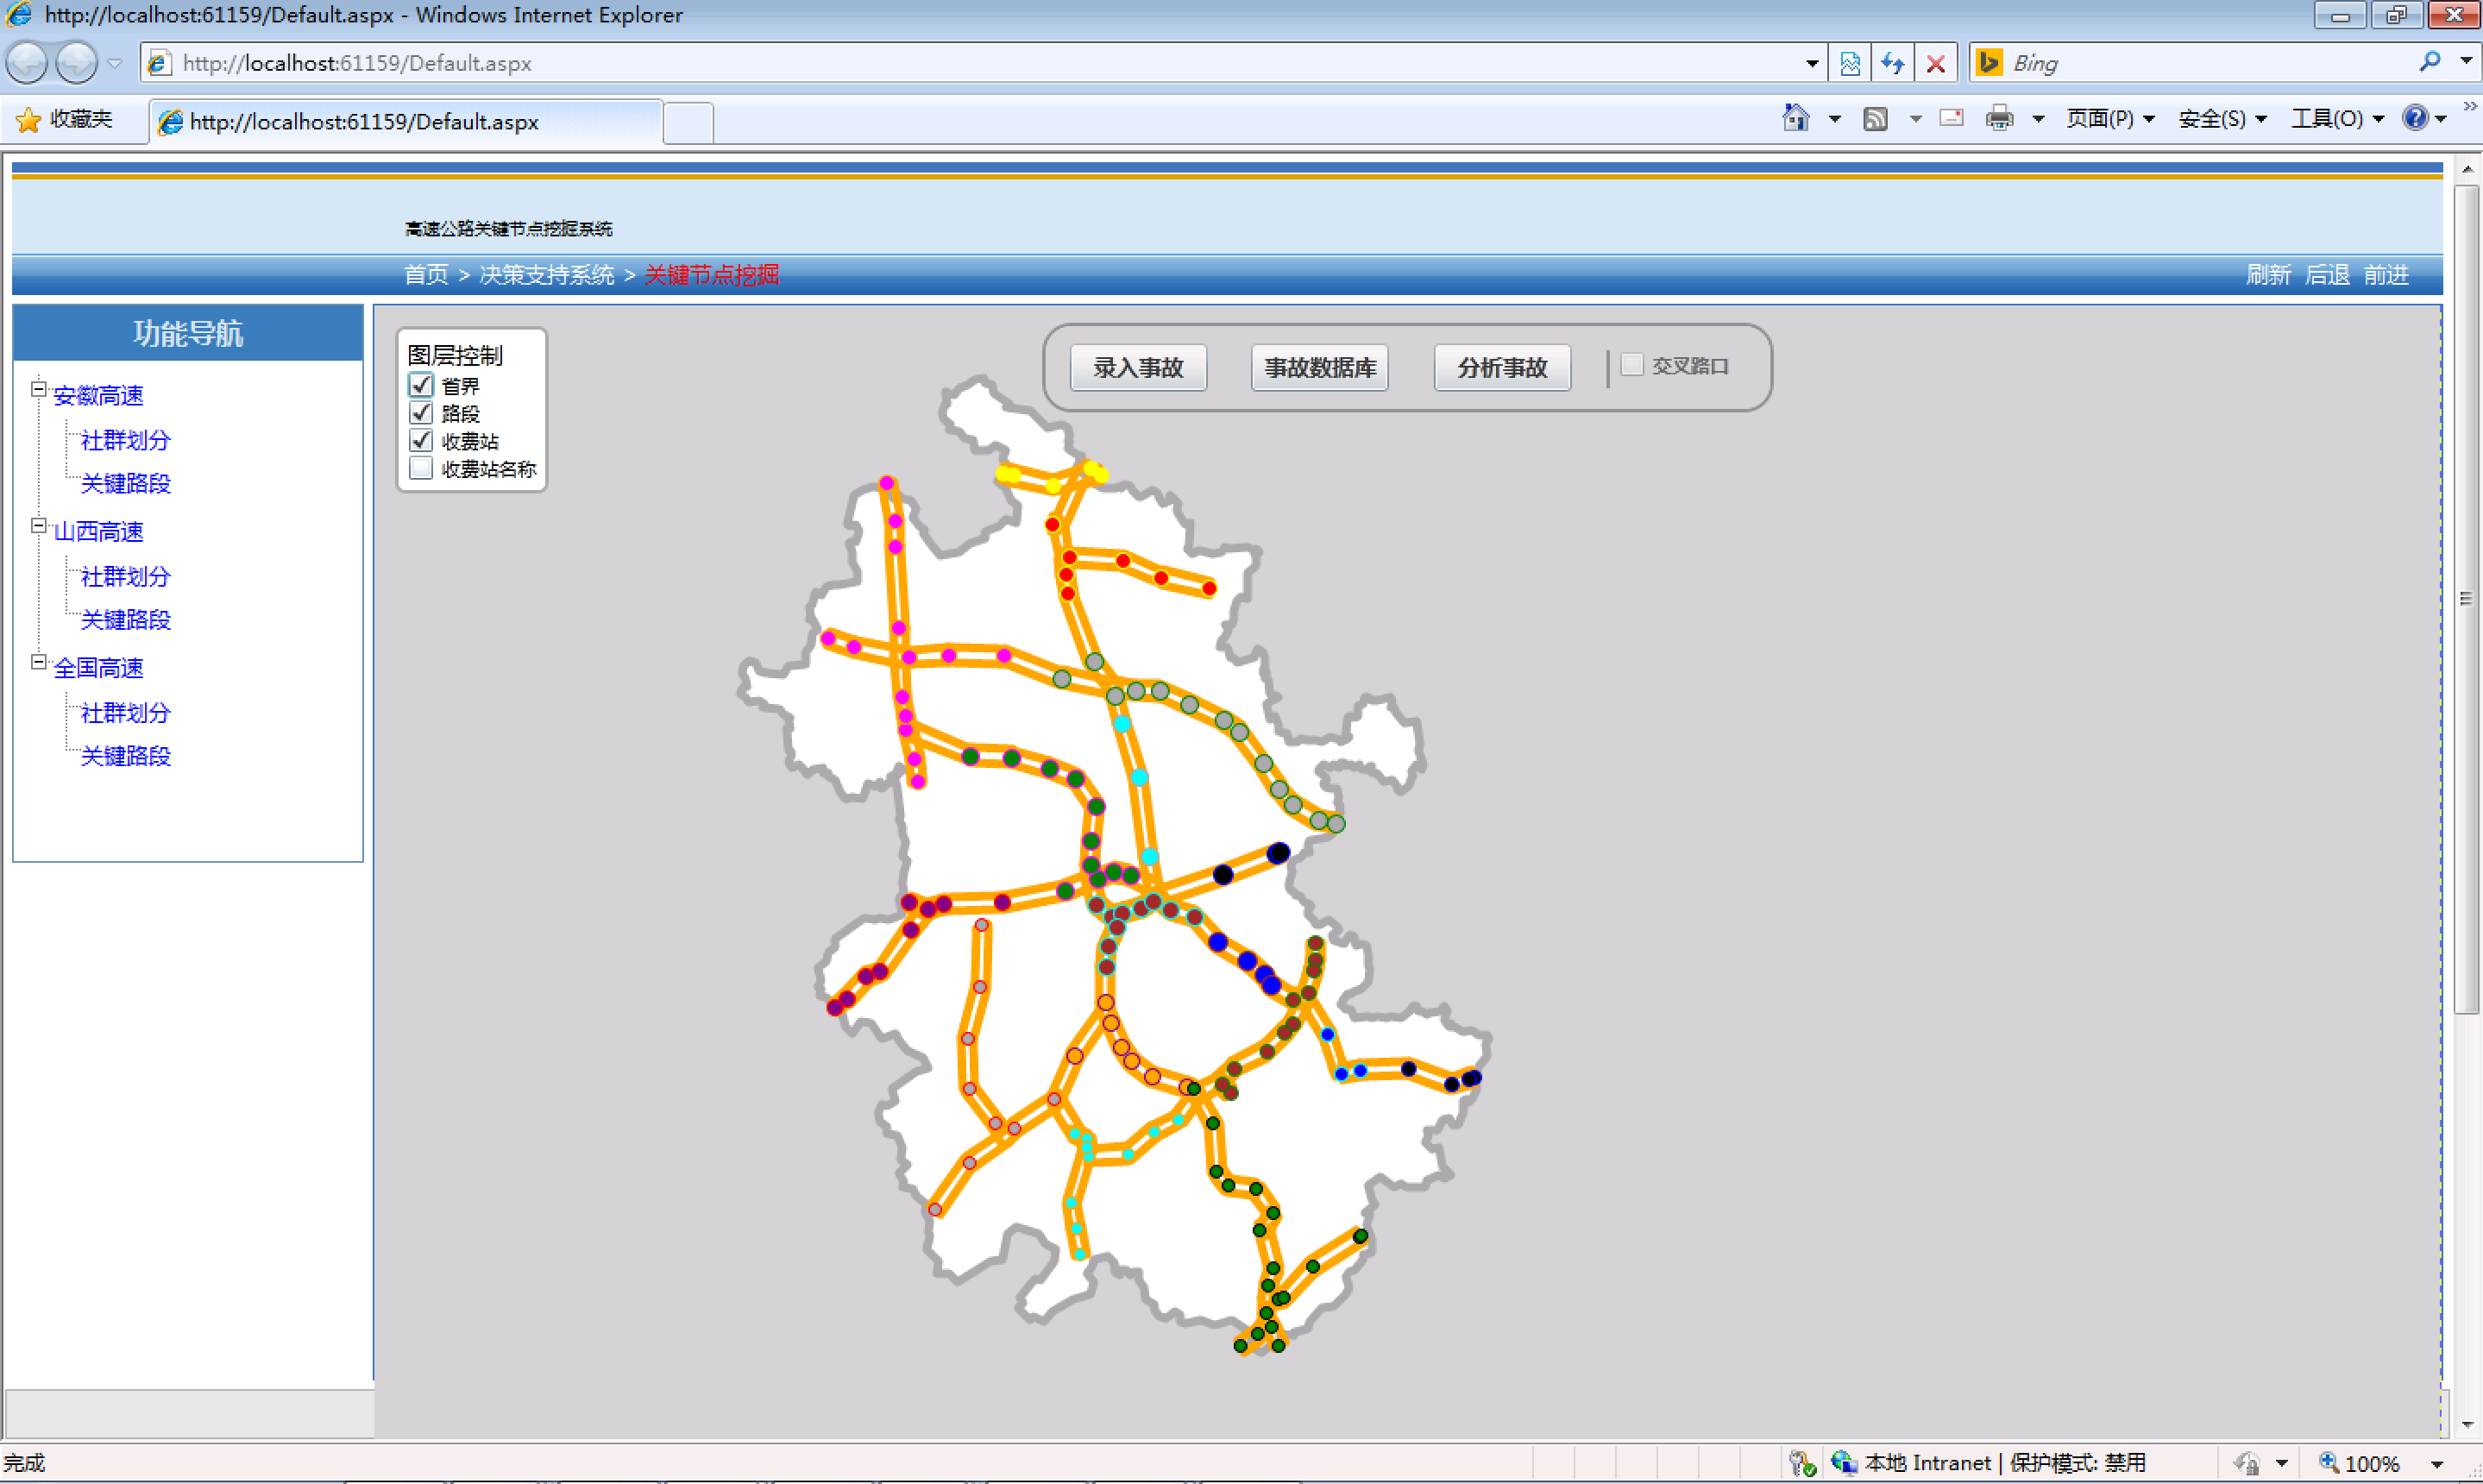
\includegraphics[width=4.4in]{picture/yuanxing1}
					\caption{fig1}
					\label{fig21}
				\end{minipage}%\
		\end{figure}


		\begin{figure}[h]
		\centering
				\begin{minipage}{0.8\linewidth}
					\centering
					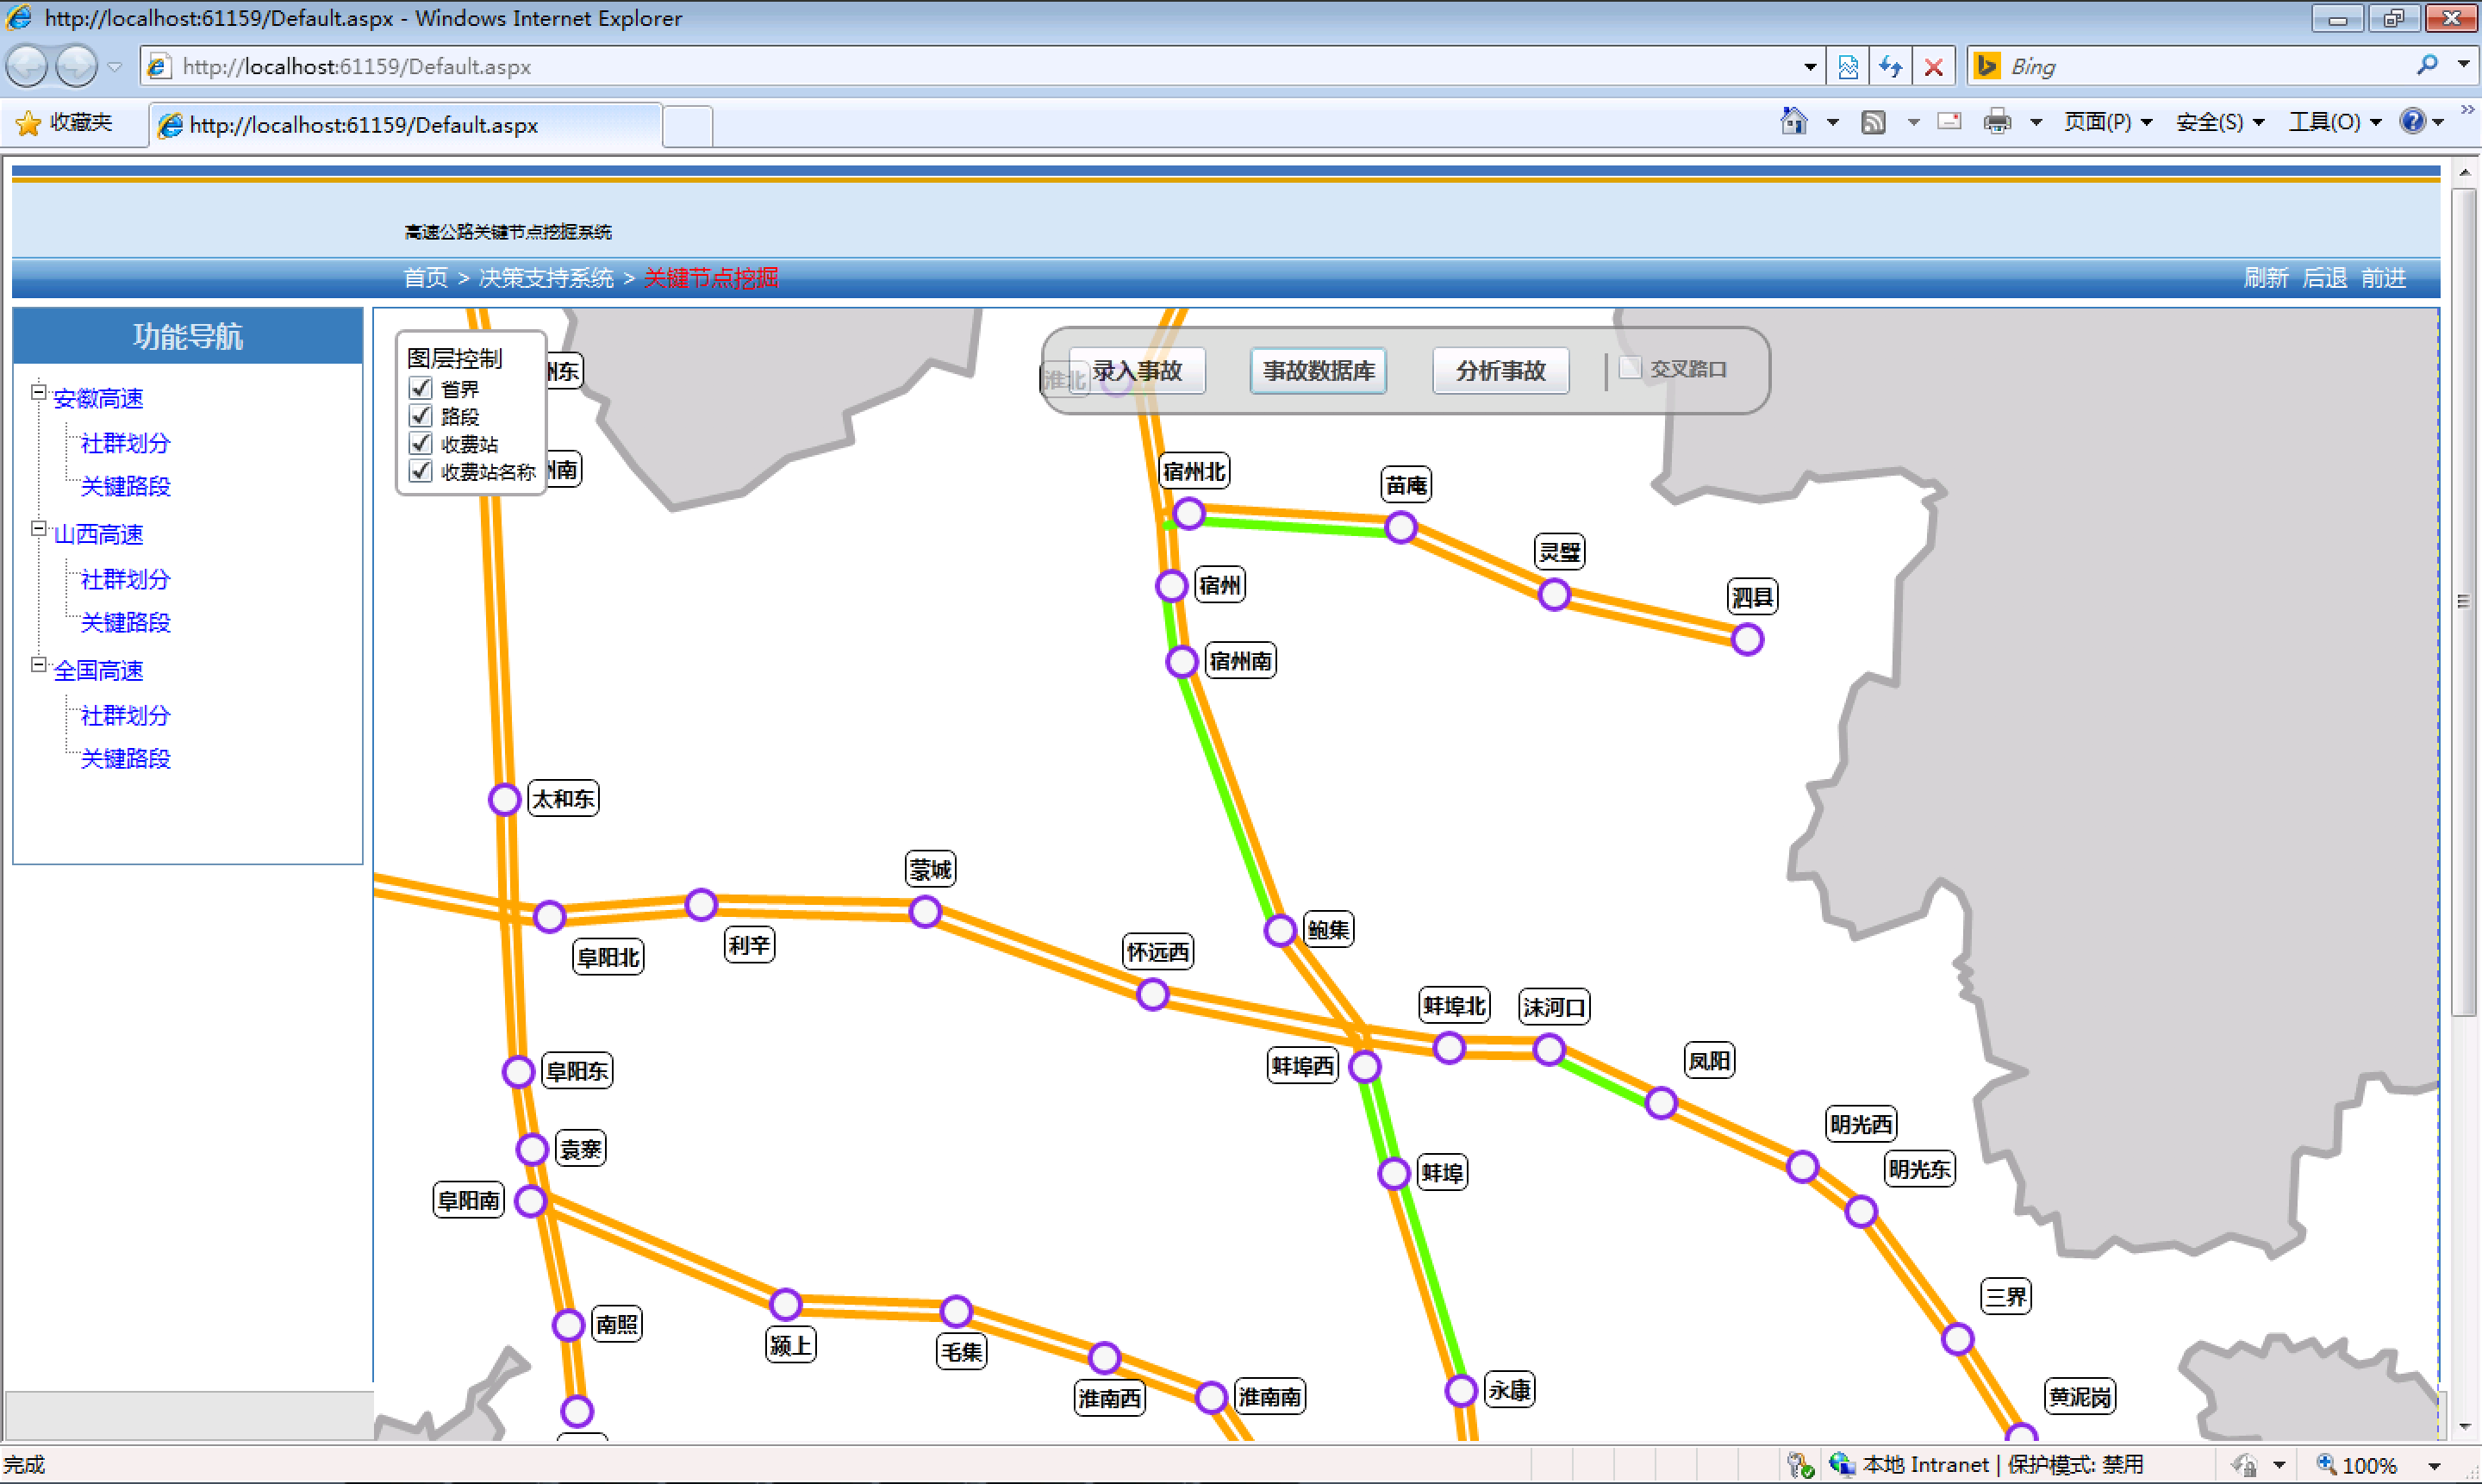
\includegraphics[width=4.4in]{picture/yuanxing2}
					\caption{fig1}
					\label{fig21}
				\end{minipage}%\
		\end{figure}

		目前系统只适用于安徽高速系统,但是系统可以扩展到任何具有收费站数据的中国高速公路上。

	\section{本章小结}
		本章介绍了一个面向高速公路的关键节点挖掘原型系统,给出了系统的流程图和样例图。该系统现在已经在安徽省高速公路网络上完全实现。该系统可扩展性强,所以可以很快的复用到其他省份乃至全国高速公路网络中。

	